\subsection{Mô hình 1 - CNN}
\subsubsection{Dữ liệu đầu vào}
Dữ liệu được chia làm 3 tập train, validation và test như sau:
\begin{lstlisting}
    from sklearn.model_selection import train_test_split
    X_train, X_test, Y_train, Y_test = train_test_split(X, Y, test_size = 0.1, random_state = 500)
    X_train, X_validate, Y_train, Y_validate = train_test_split(X_train, Y_train, test_size = 0.1, random_state = 500)
\end{lstlisting}
Thu được kích thước mỗi tập là:\\
\begin{lstlisting}
print('Train Image Data Shape: ',X_train.shape)
print('Train Label Data Shape: ',Y_train.shape)
print('Validation Image Data Shape: ',X_validate.shape)
print('Validation Label Data Shape: ',Y_validate.shape)
print('Test Image Data Shape: ',X_test.shape)
print('Test Label Data Shape: ',Y_test.shape)
\end{lstlisting}
Train Image Data Shape:  (33943, 28, 28, 1)\\
Train Label Data Shape:  (33943,)\\
Validation Image Data Shape:  (3772, 28, 28, 1)\\
Validation Label Data Shape:  (3772,)\\
Test Image Data Shape:  (4191, 28, 28, 1)\\
Test Label Data Shape:  (4191,)
\subsubsection{Xây dựng mô hình}
\begin{lstlisting}[language = python]
def build_model():
    cnn_model = Sequential()
    cnn_model.add(Conv2D(32, (3, 3), input_shape = (28,28,1), activation='relu'))
    cnn_model.add(MaxPooling2D(pool_size = (2, 2)))
    cnn_model.add(Dropout(0.25))

    cnn_model.add(Conv2D(64, (3, 3), input_shape = (28,28,1), activation='relu'))
    cnn_model.add(MaxPooling2D(pool_size = (2, 2)))
    cnn_model.add(Dropout(0.25))

    cnn_model.add(Conv2D(128, (3, 3), input_shape = (28,28,1), activation='relu'))
    cnn_model.add(MaxPooling2D(pool_size = (2, 2)))
    cnn_model.add(Dropout(0.25))

    cnn_model.add(Flatten())
    cnn_model.add(Dense(units = 64, activation = 'relu'))
    cnn_model.add(Dropout(0.25))
    cnn_model.add(Dense(units = total_class, activation = 'softmax'))
    return cnn_model
\end{lstlisting}
\newpage
\begin{center}
    \begin{figure}[!h]
        \centering
        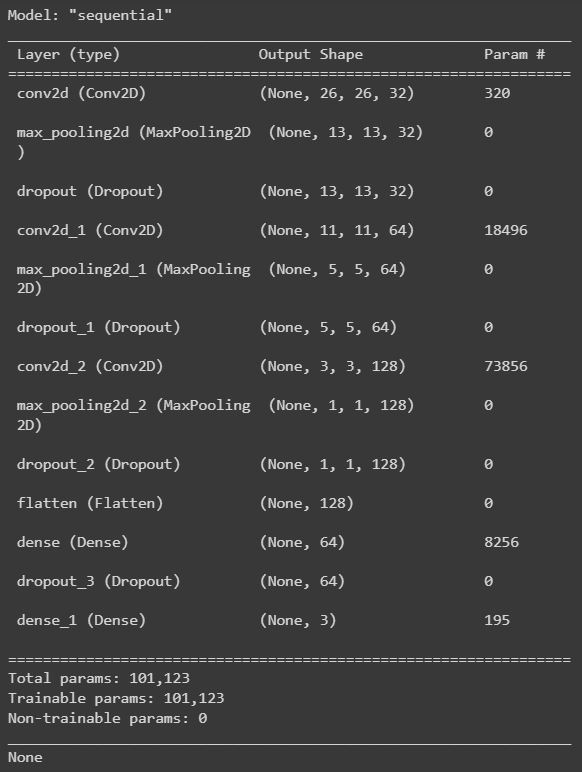
\includegraphics[scale = 0.75]{fileanh/9.jpg}
        \caption{Base model CNN}
    \end{figure}
\end{center}
\begin{lstlisting}[language = python]
def train_model(model):
    model.compile(loss ='sparse_categorical_crossentropy', optimizer='adam' ,metrics =['accuracy'])
    history = model.fit(X_train, Y_train, batch_size = 128, epochs = 50, verbose = 1, validation_data = (X_validate, Y_validate))
\end{lstlisting}

\subsubsection{kết quả training}
\begin{center}
    \begin{figure}[!h]
        \centering
        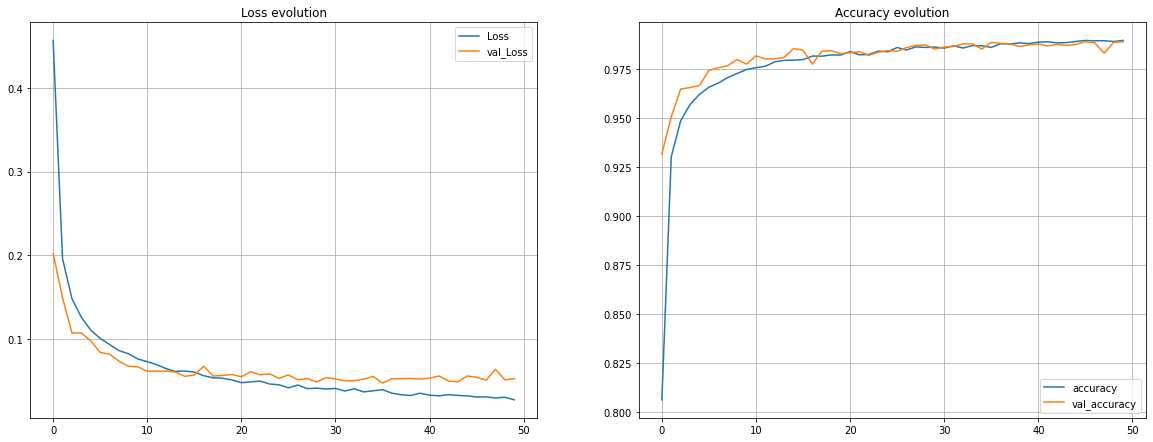
\includegraphics[scale = 0.4]{fileanh/10.png}
        \caption{Kết quả train của Base model CNN}
    \end{figure}
\end{center}

\subsubsection{Đánh giá}
Sử dụng tập test đã có với 4191 hình ảnh thì thu được ma trận nhầm lẫn như sau:
\begin{center}
    \begin{figure}[!h]
        \centering
        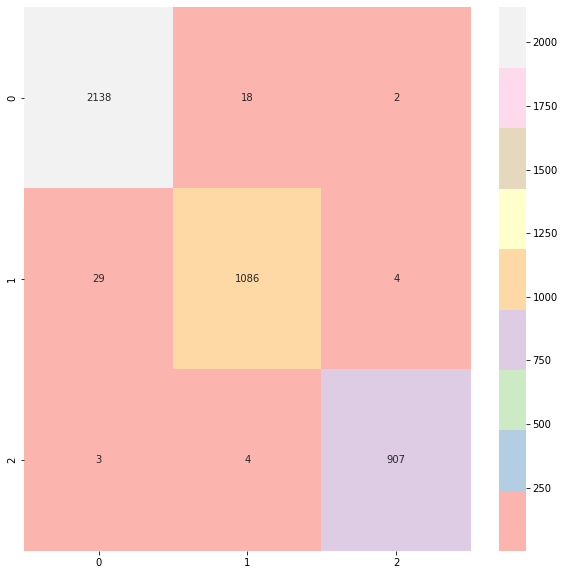
\includegraphics[scale = 0.4]{fileanh/11.png}
        \caption{Confusion matrix model 1}
    \end{figure}
\end{center}
Và các giá trị Macro average Precision, Macro average Recall, F1-score là:
\begin{center}
    \begin{figure}[!h]
        \centering
        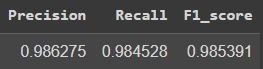
\includegraphics[scale = 1.5]{fileanh/12.jpg}
        \caption{Các chỉ số đánh giá model 1}
    \end{figure}
\end{center}

%\begin{block}{Nhận xét}
%Các chỉ số đánh giá khá cao tuy nhiên vẫn chưa thể coi đây là 1 model tốt bởi có thể do lượng dữ liệu đầu vào khá ít hoặc có thể trùng nhau.
%\end{block}

\newpage

\subsection{Mô hình 2 - CNN}
\subsubsection{Dữ liệu đầu vào }
Sử dụng \textbf{ImageDataGenerator} chia dữ liệu thành 2 tập là training\_generator và validation\_generator
\begin{lstlisting}
from keras.preprocessing.image import ImageDataGenerator

#image generator object from keras. reference : Keras Docs
image_generator = ImageDataGenerator(
    validation_split=0.2
)

#create a flow of images for training the model.
training_generator = image_generator.flow_from_dataframe(
    dataframe = df,
    directory= "/content/drive/MyDrive/myntradataset/images/",
    x_col="image",
    y_col="masterCategory",
    target_size=(224,224),
    batch_size=32,
    subset="training"

)

#create a flow of images for validating(testing) the trained model.
validation_generator = image_generator.flow_from_dataframe(
    dataframe = df,
    directory="/content/drive/MyDrive/myntradataset/images/",
    x_col="image",
    y_col="masterCategory",
    target_size=(224,224),
    batch_size=32,
    subset="validation"
)
\end{lstlisting}
Found 33525 validated image filenames belonging to 3 classes.\\
Found 8381 validated image filenames belonging to 3 classes.\\

Còn tập test sẽ đc lấy ra một phần từ tập validation\_generator như sau:
\begin{lstlisting}
batch_size = 32
#!pip install tqdm
import tqdm
validation_generator.reset()
X_test, y_test = next(validation_generator)
for i in tqdm.tqdm(range(int(validation_generator.n/batch_size)-200)): 
  img, label = next(validation_generator)
  X_test = np.append(X_test, img, axis=0 )
  y_test = np.append(y_test, label, axis=0)
print(X_test.shape, y_test.shape)
\end{lstlisting}
Thu được tập test gồm có 1984 hình ảnh và nhãn của nó.

\subsubsection{Xây dựng mô hình}
%So với mô hình 1 thì mô hình thứ 2 này tuy vẫn dùng CNN nhưng cấu trúc nó thì được thay đổi, kể cả việc đưa dữ liệu đầu vào cũng đc xử lý theo một cách khác với target\_size là 224
\begin{lstlisting}
from keras import layers,models
model1 = Sequential()
model1.add(layers.Conv2D(16, (4,4),  activation = 'relu' , input_shape = (224,224,3)))
model1.add(MaxPooling2D(pool_size = (2, 2)))

model1.add(Conv2D(32, (3,3), activation='relu'))
model1.add(MaxPooling2D(pool_size = (2, 2)))

model1.add(Conv2D(64, (3,3), activation='relu'))
model1.add(MaxPooling2D(pool_size = (2, 2)))

model1.add(Conv2D(64, (3,3), activation='relu'))
model1.add(MaxPooling2D(pool_size = (2, 2)))

model1.add(Conv2D(128, (3,3), activation='relu'))
model1.add(MaxPooling2D(pool_size = (2, 2)))


model1.add(Flatten())
model1.add(Dense(units=512, activation='relu'))
model1.add(Dropout(0.25))
model1.add(Dense(units=256, activation='relu'))
model1.add(Dropout(0.25))
model1.add(Dense(units=128, activation='relu'))
model1.add(Dropout(0.25))
model1.add(Dense(units=3, activation='softmax'))

model1.compile(optimizer='adam',
              loss='categorical_crossentropy',
              metrics=['accuracy'])

model1.summary()
\end{lstlisting}
\newpage
\begin{center}
    \begin{figure}[!h]
        \centering
        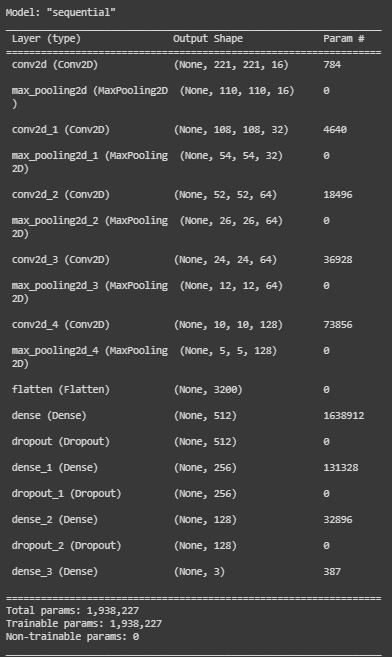
\includegraphics[scale = 1.2]{fileanh/13.jpg}
        \caption{Model 2}
    \end{figure}
\end{center}
\subsubsection{Kết quả training}
\begin{center}
    \begin{figure}[!h]
        \centering
        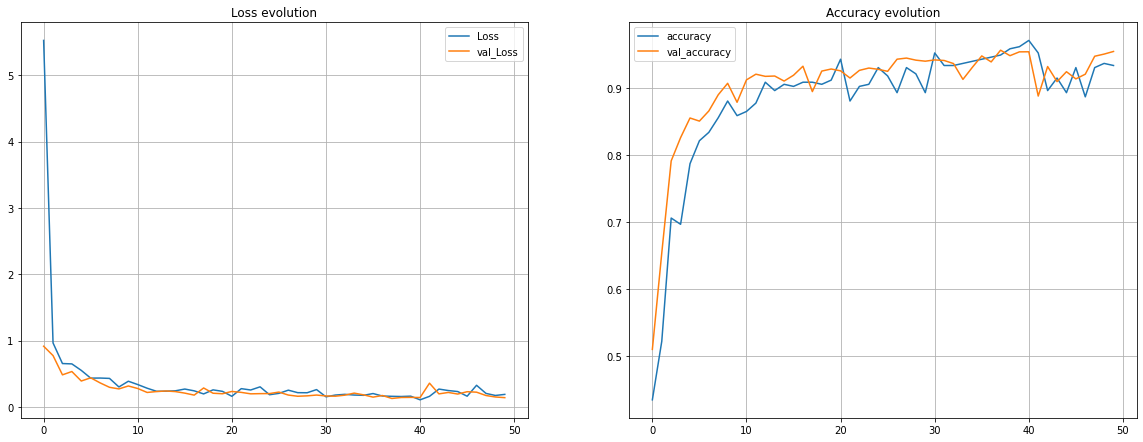
\includegraphics[scale = 0.4]{fileanh/14.png}
        \caption{Kết quả train của Model 2}
    \end{figure}
\end{center}

\subsubsection{Đánh giá}
Với 1984 hình ảnh ta thu được các giá trị của ma trận nhầm lẫn:
\begin{center}
    \begin{figure}[!h]
        \centering
        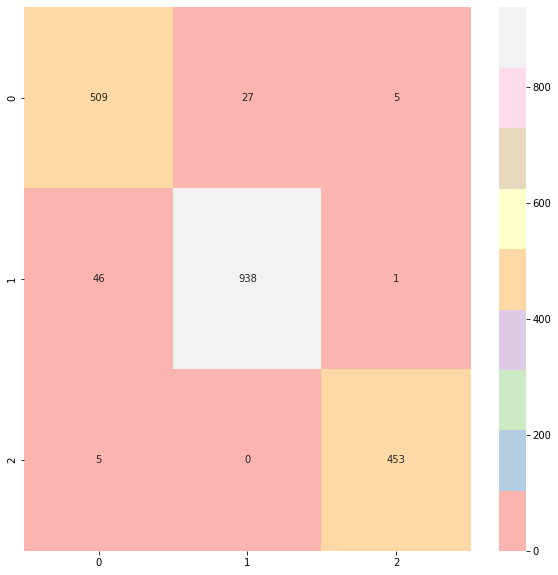
\includegraphics[scale = 0.4]{fileanh/15.png}
        \caption{Confusion matrix của Model 2}
    \end{figure}
\end{center}
Và các giá trị Macro average Precision, Macro average Recall, F1-score là:
\begin{center}
    \begin{figure}[!h]
        \centering
        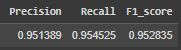
\includegraphics[scale = 2.5]{fileanh/16.jpg}
        \caption{Các chỉ số đánh giá của Model 2}
    \end{figure}
\end{center}
%\begin{block}{Nhận xét}
%Với việc thay đổi cách chia dữ liệu đầu vào và thay đổi một chút cấu trúc của model thì các chỉ số %đánh giá giảm hơn đôi chút so với model 1 nhưng cũng vẫn khá cao.
%\end{block}

\newpage
\subsection{Mô hình 4 - VGG16}
\subsubsection{Dữ liệu đầu vào}
Tương tự như mô hình 2
\subsubsection{Xây dựng mô hình}
\begin{lstlisting}
image_size=[227,227]
model=VGG16(input_shape=image_size+[3],include_top=False,weights="imagenet")
\end{lstlisting}
\begin{lstlisting}
for layers in model.layers:
  layers.trainable=False
\end{lstlisting}
Thêm một số layers cần thiết
\begin{lstlisting}
final_model=Model(inputs=model.input,outputs=Dense(3,activation="softmax")(Flatten()(model.output)))
final_model.summary()
\end{lstlisting}

\begin{center}
    \begin{figure}[!h]
        \centering
        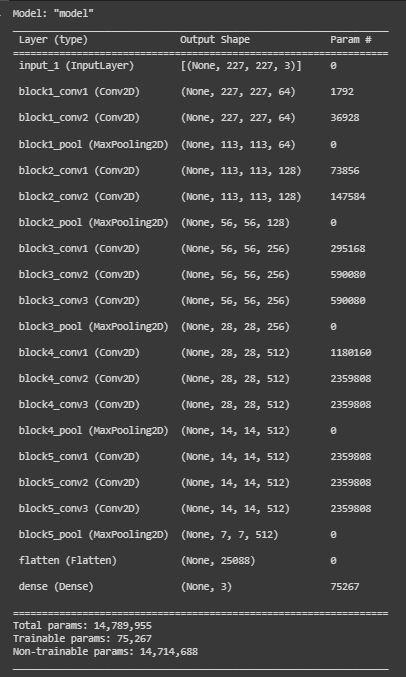
\includegraphics[scale = 1]{fileanh/20.jpg}
        \caption{Model VGG16}
    \end{figure}
\end{center}

\begin{lstlisting}
final_model.compile(loss="binary_crossentropy",optimizer="adam",metrics=['accuracy'])  
vgg16=final_model.fit(training_generator,epochs=50,steps_per_epoch=20,validation_data=validation_generator)
\end{lstlisting}

\subsubsection{Kết quả training}
\begin{center}
    \begin{figure}[!h]
        \centering
        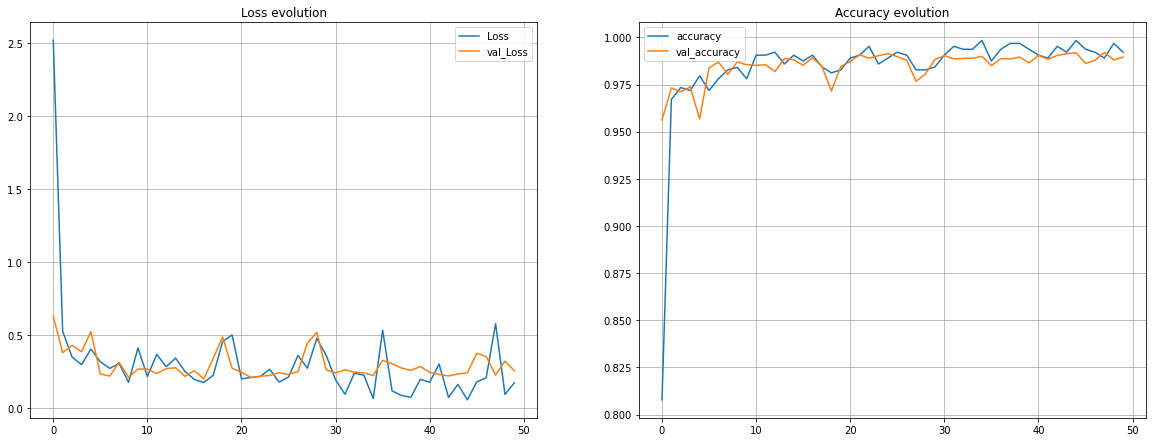
\includegraphics[scale = 0.4]{fileanh/21.png}
        \caption{kết quả train của Model VGG16}
    \end{figure}
\end{center}
\subsubsection{Đánh giá}
Các giá trị trên ma trận nhầm lẫn:
%\newpage
\begin{center}
    \begin{figure}[!h]
        \centering
        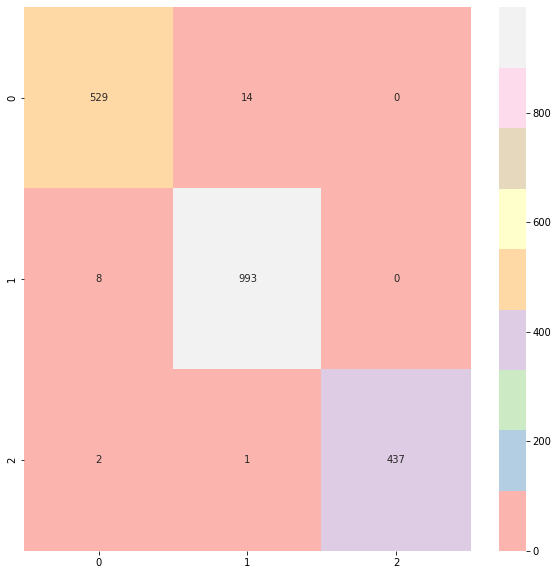
\includegraphics[scale = 0.4]{fileanh/22.png}
        \caption{Confusion matrix của Model VGG16}
    \end{figure}
\end{center}
Và các giá trị Macro average Precision, Macro average Recall, F1-score là:
\begin{center}
    \begin{figure}[!h]
        \centering
        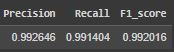
\includegraphics[scale = 2]{fileanh/23.jpg}
        \caption{Chỉ số đánh giá của Model VGG16}
    \end{figure}
\end{center}

%\begin{block}{Nhận xét}
    
%\end{block}



\newpage


\subsection{Mô hình 8 - Alexnet} 
\subsubsection{Dữ liệu đầu vào}
Tương tự như mô hình 2
\subsubsection{Xây dựng mô hình}
\begin{lstlisting}
model=Sequential()
model.add(Conv2D(filters=96,strides=(4,4),kernel_size=(11,11),padding='valid',input_shape=(227,227,3),activation='relu'))
model.add(BatchNormalization())
model.add(MaxPooling2D(pool_size=(3,3),strides=(2,2)))
model.add(Conv2D(filters=256,strides=(1,1),kernel_size=(5,5),padding='valid',activation='relu'))
model.add(MaxPooling2D(pool_size=(3,3),strides=(2,2)))
model.add(Conv2D(filters=384,kernel_size=(3,3),strides=(1,1),padding='valid',activation='relu'))
model.add(BatchNormalization())
model.add(Conv2D(filters=384,kernel_size=(3,3),strides=(1,1),padding='valid',activation='relu'))
model.add(BatchNormalization())
model.add(Conv2D(filters=256,kernel_size=(3,3),strides=(1,1),padding='valid',activation='relu'))
model.add(BatchNormalization())
model.add(MaxPooling2D(pool_size=(3,3),strides=(2,2),padding='valid'))
model.add(Flatten())
model.add(Dense(units=4096,activation='relu'))
model.add(Dropout(0.2))
model.add(Dense(units=4096,activation='relu'))
model.add(Dropout(0.2))
model.add(Dense(units=3,activation='softmax')) 
\end{lstlisting}

\begin{lstlisting}
model.compile(loss='binary_crossentropy', optimizer='adam', metrics=['accuracy']) 
alexnet_model=model.fit(training_generator,epochs=50,validation_data=validation_generator,steps_per_epoch=len(training_generator),validation_steps=len(validation_generator))
\end{lstlisting}

\newpage
\begin{center}
    \begin{figure}[!h]
        \centering
        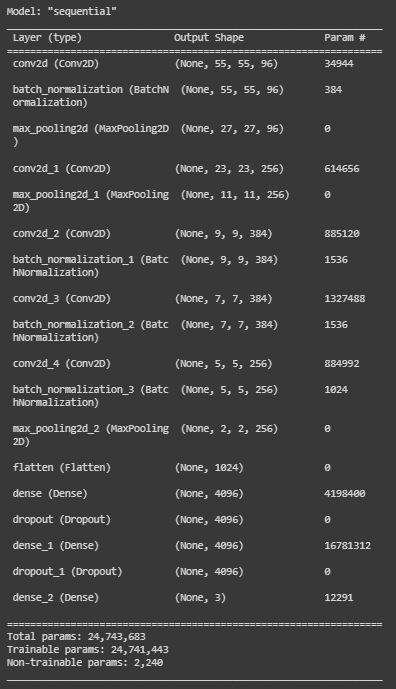
\includegraphics[scale = 1]{fileanh/33.jpg}
        \caption{Model Alexnet}
    \end{figure}
\end{center}



\subsubsection{Kết quả training}
\begin{center}
    \begin{figure}[!h]
        \centering
        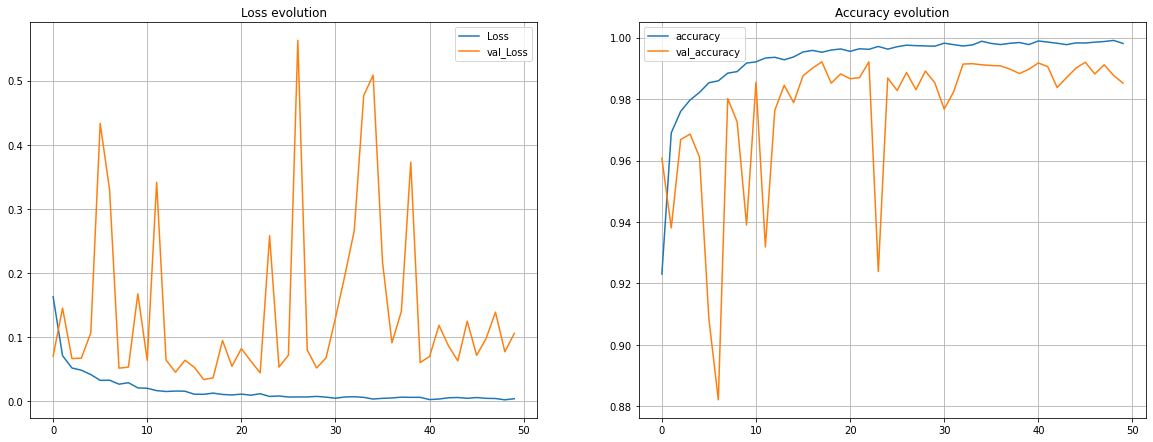
\includegraphics[scale = 0.4]{fileanh/34.png}
        \caption{kết quả train của Model Alexnet}
    \end{figure}
\end{center}
\subsubsection{Đánh giá}
Các giá trị trên ma trận nhầm lẫn:
%\newpage
\begin{center}
    \begin{figure}[!h]
        \centering
        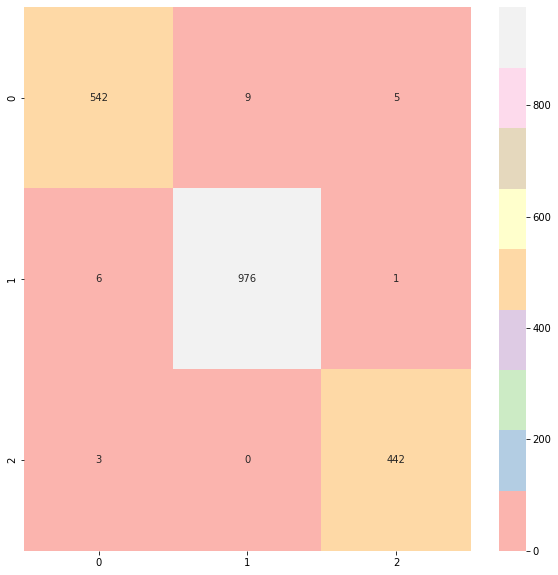
\includegraphics[scale = 0.4]{fileanh/35.png}
        \caption{Confusion matrix của Model Alexnet}
    \end{figure}
\end{center}
Và các giá trị Macro average Precision, Macro average Recall, F1-score là:
\begin{center}
    \begin{figure}[!h]
        \centering
        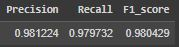
\includegraphics[scale = 2]{fileanh/36.jpg}
        \caption{Chỉ số đánh giá của Model Alexnet}
    \end{figure}
\end{center}

%\begin{block}{Nhận xét}
    
%\end{block}
\newpage







\subsection{Mô hình 10 - Resnet101}
\subsubsection{Dữ liệu đầu vào}
Tương tự như mô hình 2
\subsubsection{Xây dựng mô hình}
\begin{lstlisting}
image_size=[227,227]
model=ResNet101(input_shape=image_size+[3],include_top=False,weights="imagenet")
\end{lstlisting}
\begin{lstlisting}
for layers in model.layers:
  layers.trainable=False
\end{lstlisting}
Thêm một số layers cần thiết
\begin{lstlisting}
final_model=Model(inputs=model.input,outputs=Dense(3,activation="softmax")(Flatten()(model.output)))
final_model.summary()
\end{lstlisting}

\begin{center}
    \begin{figure}[!h]
        \centering
        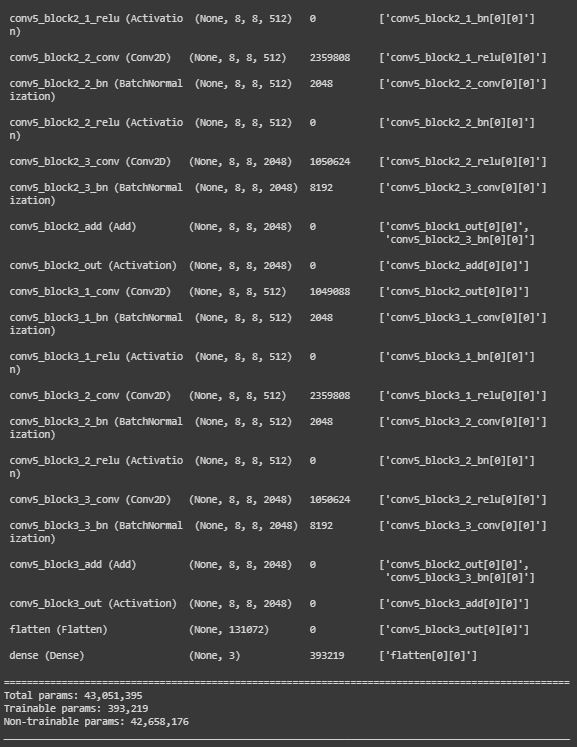
\includegraphics[scale = 1]{fileanh/37.jpg}
        \caption{Model Resnet101}
    \end{figure}
\end{center}

\begin{lstlisting}
from tensorflow.keras.optimizers import RMSprop
final_model.compile(loss="categorical_crossentropy",optimizer=RMSprop(lr=0.001),metrics=['accuracy'])
resnet = final_model.fit(training_generator,epochs=50,steps_per_epoch=20,validation_data=validation_generator)
\end{lstlisting}

\subsubsection{Kết quả training}
\begin{center}
    \begin{figure}[!h]
        \centering
        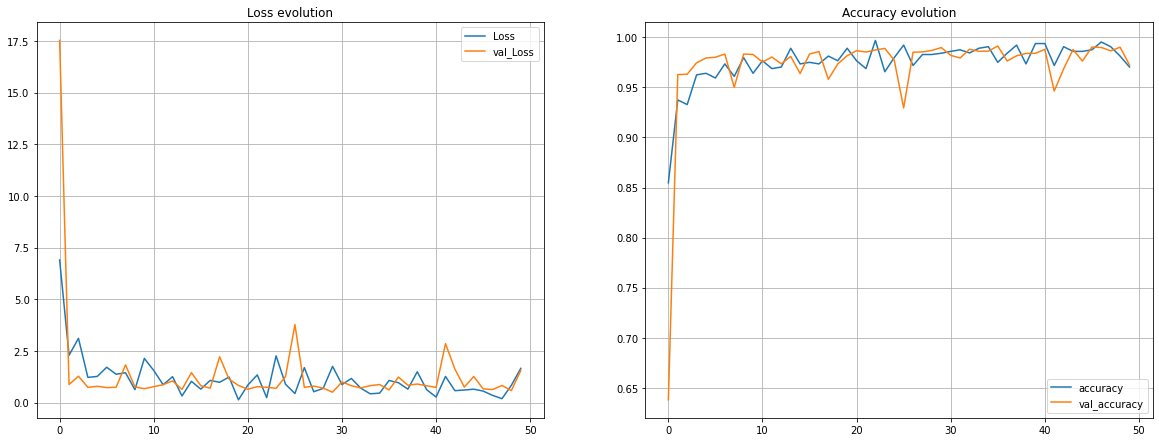
\includegraphics[scale = 0.4]{fileanh/38.png}
        \caption{kết quả train của Model Resnet101}
    \end{figure}
\end{center}
\subsubsection{Đánh giá}
Các giá trị trên ma trận nhầm lẫn:
%\newpage
\begin{center}
    \begin{figure}[!h]
        \centering
        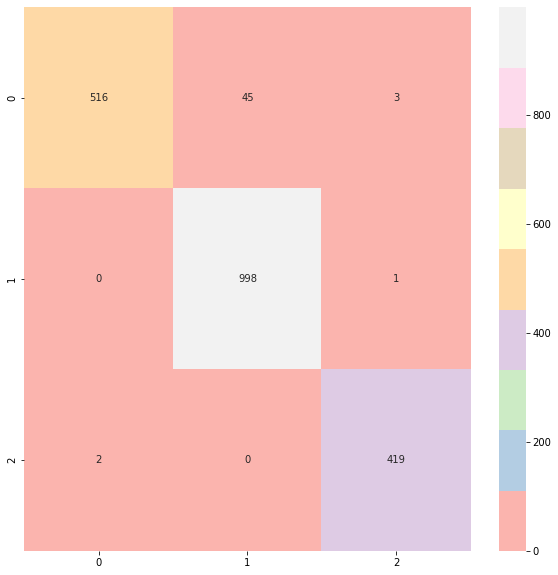
\includegraphics[scale = 0.35]{fileanh/39.png}
        \caption{Confusion matrix của Model Resnet101}
    \end{figure}
\end{center}
Và các giá trị Macro average Precision, Macro average Recall, F1-score là:
\begin{center}
    \begin{figure}[!h]
        \centering
        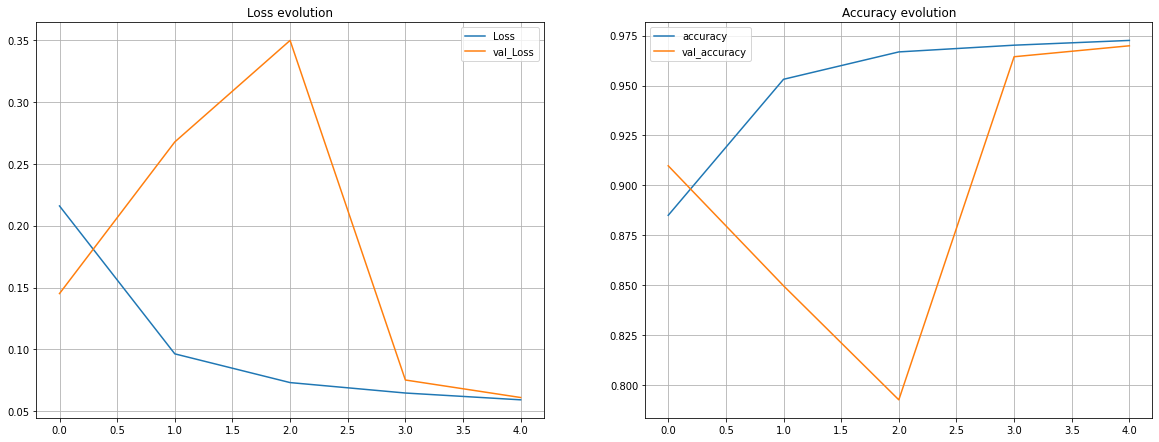
\includegraphics[scale = 2]{fileanh/40.jpg}
        \caption{Chỉ số đánh giá của Model Resnet101}
    \end{figure}
\end{center}

%\begin{block}{Nhận xét}
    
%\end{block}
